\section{The \sysname Framework}
\label{sec:framework}

We now detail the three layers of \sysname:
the \clsm and its on-chain instantiation (\S~\ref{sec:framework-clsm}),
the Verifiable Unlearning Protocol with its three MIA components
(\S~\ref{sec:framework-vup}), and the three-contract Solidity
architecture that closes the automation loop
(\S~\ref{sec:framework-contracts}).
Figure~\ref{fig:arch} gives the layered overview.

\begin{figure}[t]
\centering
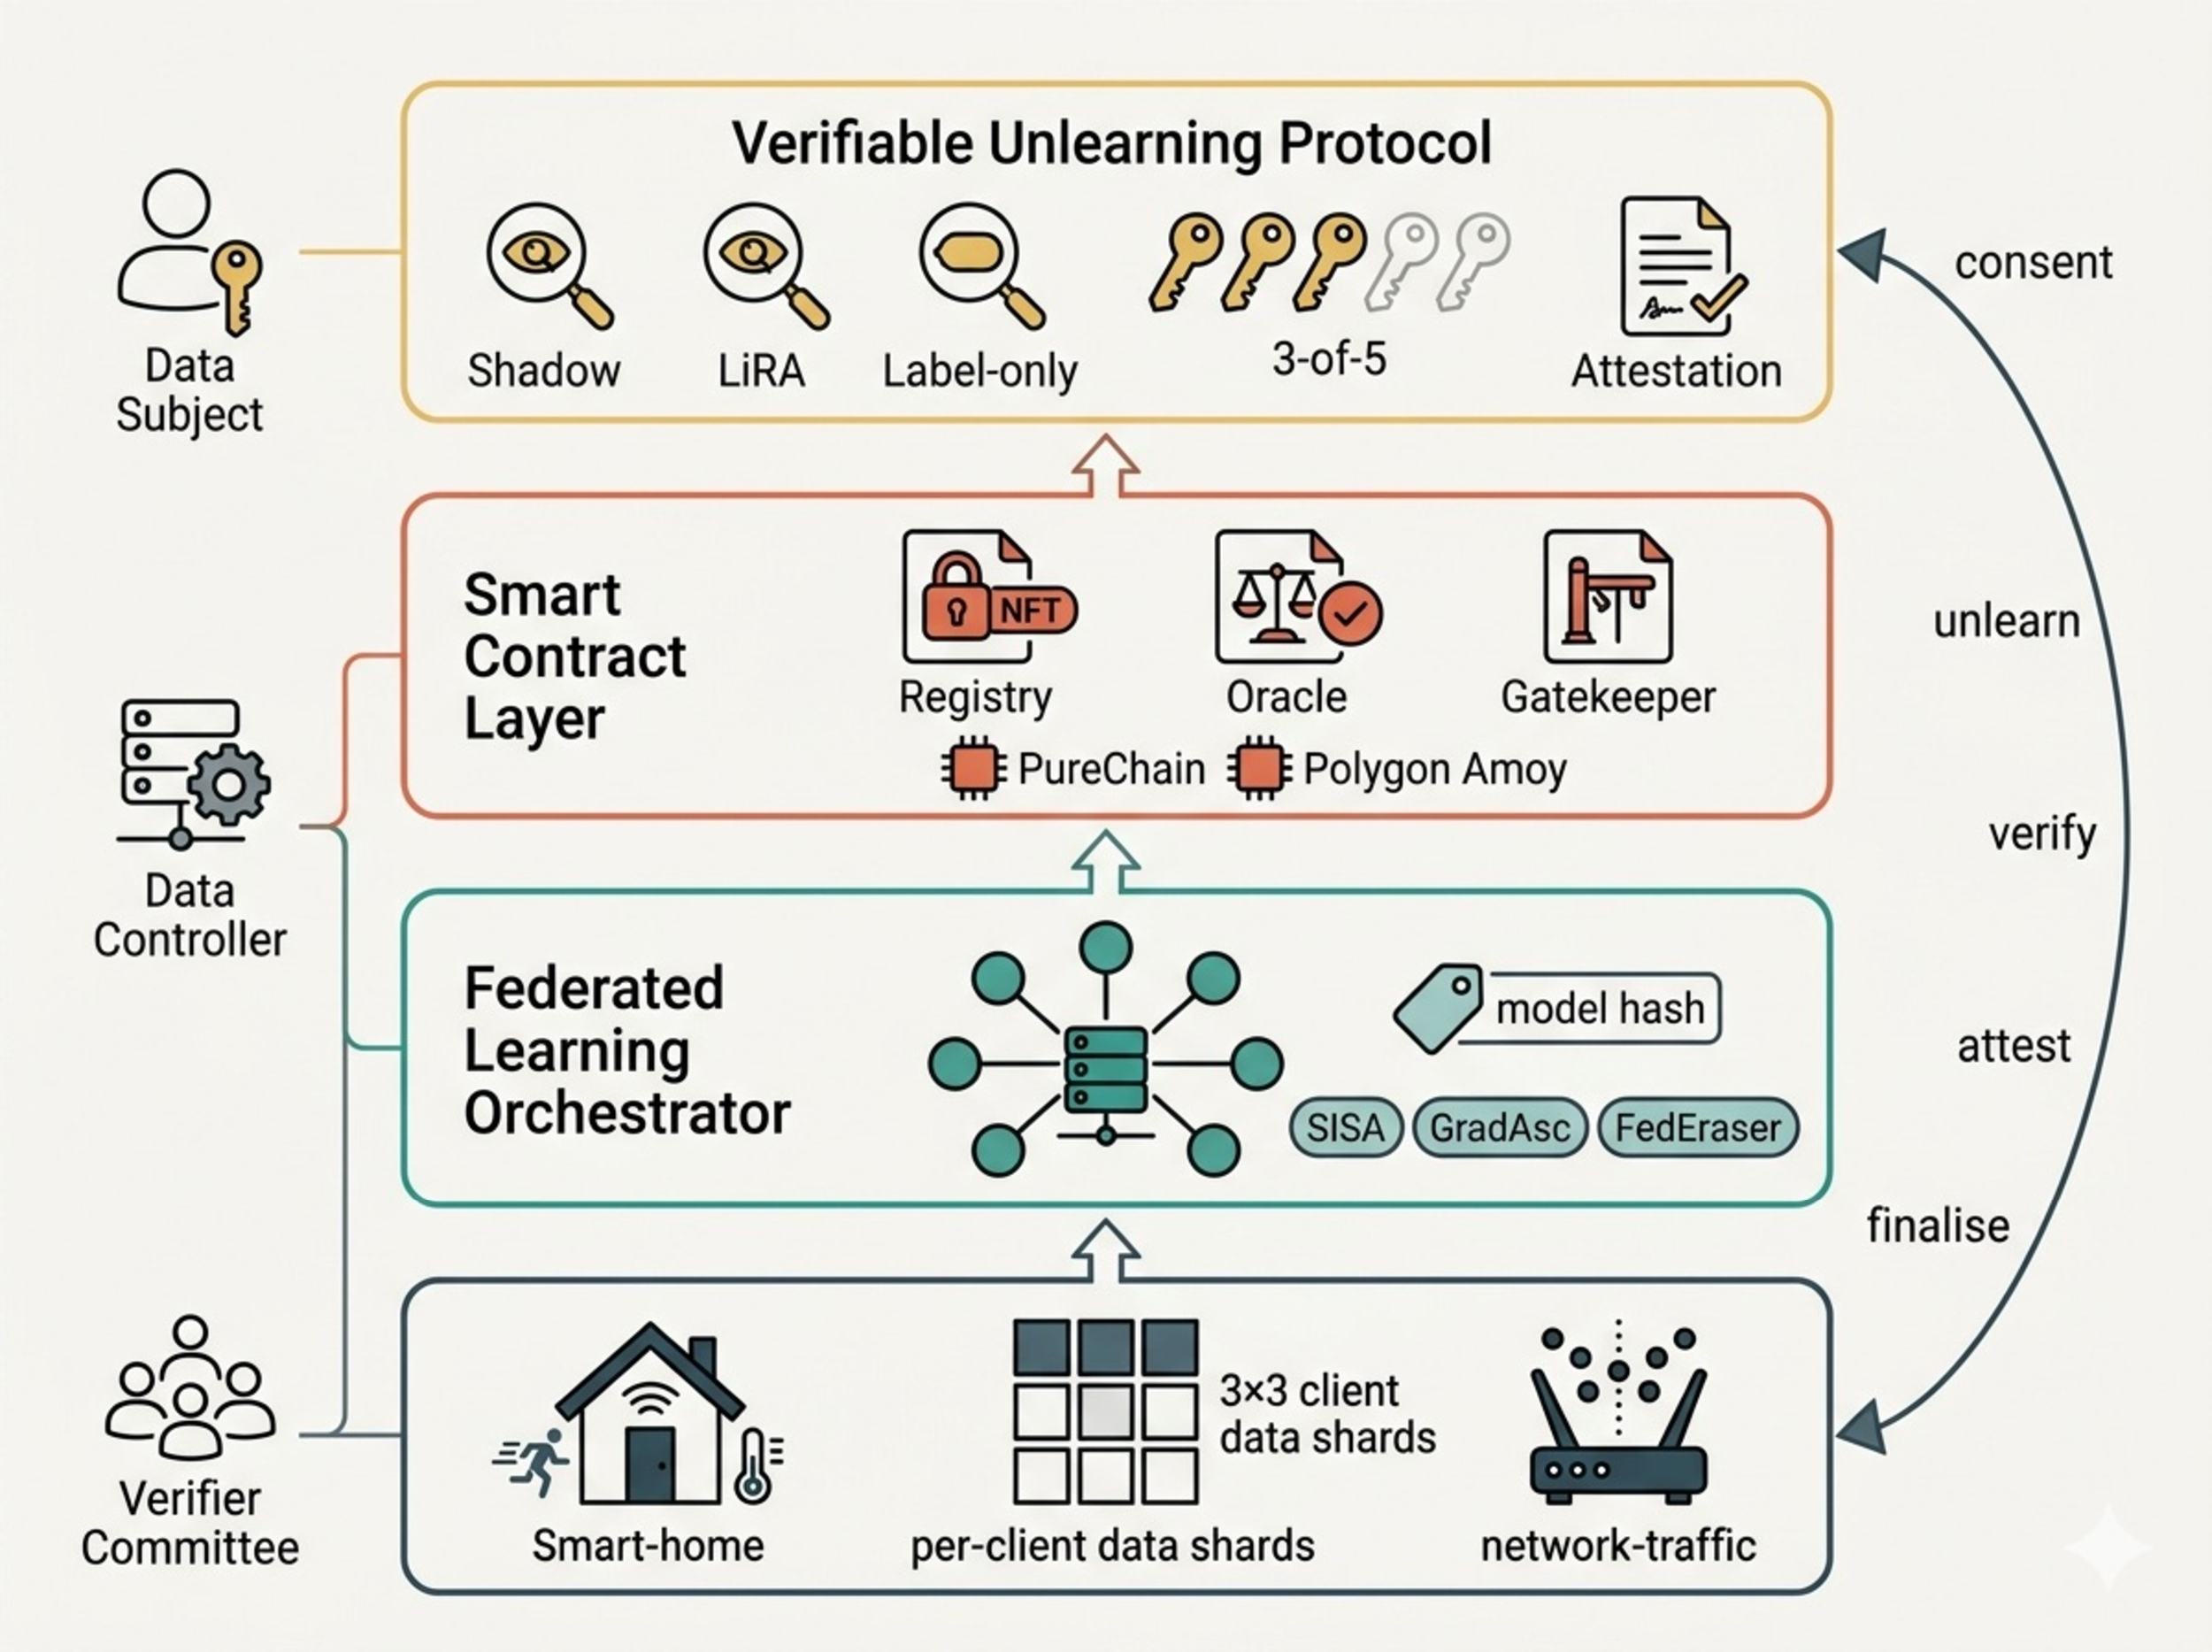
\includegraphics[width=0.96\columnwidth]{figures/system_architecture.pdf}
\caption{\sysname architecture: off-chain IoT data and Flower
FedAvg layers, the three on-chain Solidity contracts on PureChain /
Polygon Amoy, and the off-chain Verifiable Unlearning Protocol. The
clockwise loop consent$\rightarrow$unlearn$\rightarrow$verify
$\rightarrow$attest$\rightarrow$finalise is the edge \sysname closes.}
\label{fig:arch}
\end{figure}

\subsection{Consent Lifecycle State Machine}
\label{sec:framework-clsm}

The \clsm transition function $\delta$ from Definition~\ref{def:clsm}
is summarised in Table~\ref{tab:clsm}. Five edges are
$\mathit{DS}_i$-controlled (\texttt{grant}, \texttt{modify},
\texttt{suspend}, \texttt{resume}, \texttt{revoke}); two are
time-driven (\texttt{tick}, \texttt{expire}); one
(\texttt{unlearn\_verified}) is callable only by the
\texttt{UnlearningOracle} after a valid UA submission. The
\textsc{Unlearned} state has no outgoing edges, making it absorbing.

\begin{table}[t]
\centering
\caption{\clsm transition table. \texttt{rev} = \texttt{revoke},
\texttt{susp} = \texttt{suspend}, \texttt{uv} =
\texttt{unlearn\_verified}.}
\label{tab:clsm}
\small
\begin{tabular}{l@{\hspace{4pt}}l@{\hspace{4pt}}l@{\hspace{4pt}}l}
\toprule
Current & Event & Next & Guard \\
\midrule
\textsc{Inactive}  & \texttt{grant}($\mathcal{P},T$) & \textsc{Active}($\mathcal{P},T$) & DS signature \\
\textsc{Active}    & \texttt{modify}($\mathcal{P}',T'$) & \textsc{Active}($\mathcal{P}',T'$) & DS signature \\
\textsc{Active}    & \texttt{susp}() & \textsc{Suspended} & DS signature \\
\textsc{Active}    & \texttt{tick}($r$) & \textsc{Active} & $\rho_r \!\in\!\mathcal{P}$, $T\!>\!b$ \\
\textsc{Active}    & \texttt{rev}($\mathcal{P}'$) & \textsc{Revoked}($\mathcal{P}'$) & DS signature \\
\textsc{Active}    & \texttt{expire}() & \textsc{Expired} & $b\!>\!T$ \\
\textsc{Suspended} & \texttt{resume}() & \textsc{Active} & DS signature \\
\textsc{Revoked}   & \texttt{uv}() & \textsc{Unlearned} & valid UA on-chain \\
\textsc{Expired}   & \texttt{uv}() & \textsc{Unlearned} & valid UA on-chain \\
\bottomrule
\end{tabular}
\end{table}

Property~\ref{prop:safety} follows by inspection of
Table~\ref{tab:clsm}: there is no edge into \textsc{Active} from
\textsc{Revoked} or \textsc{Expired}, and the
$\mathtt{tick}(r)$ self-edge guards on $\rho_r \in \mathcal{P}$.
The \texttt{validateRound} function (\S~\ref{sec:framework-contracts})
fires only the $\mathtt{tick}$ edge.

\subsection{Verifiable Unlearning Protocol}
\label{sec:framework-vup}

When a token transitions to \textsc{Revoked} or \textsc{Expired}, the
gatekeeper records $\mathtt{pendingUnlearningSince}[i] = b$ and
\texttt{validateRound} blocks all future rounds
(Property~\ref{prop:liveness}). The data controller has until
$b + \dmax$ to (i) execute an unlearning procedure, (ii) collect
three MIA scores from the post-unlearning model, (iii) assemble the
Unlearning Attestation, (iv) gather $t$-of-$n$ verifier signatures,
and (v) submit it on-chain.

\subsubsection{Approximate unlearning methods}

\sysname is method-agnostic. We evaluate three established families:

\paragraph{SISA-Fed} pre-shards each client's data into $S$ disjoint
shards and caches a per-shard intermediate
checkpoint~\cite{bourtoule2021sisa}. Unlearning a revoked client
$\mathit{DS}_i$ reduces to retraining only the shards that touched
$i$'s data, then re-aggregating.

\paragraph{Gradient ascent} performs $k$ steps of negative-learning-rate
gradient ascent on the cached gradients of the revoked client:
\begin{equation}\label{eq:gradascent}
    \theta^{(j+1)} \;=\; \theta^{(j)} \;+\; \eta \,\nabla
        \mathcal{L}\!\left(\theta^{(j)}; \mathcal{D}_i\right),
    \quad j = 0, 1, \ldots, k\!-\!1,
\end{equation}
where $\mathcal{D}_i$ is $\mathit{DS}_i$'s local training set,
$\mathcal{L}$ is the FL loss (here mean-squared reconstruction error
for the N-BaIoT autoencoder), and $\eta > 0$ is the unlearning rate.
We use $k=10$, $\eta = 10^{-4}$.

\paragraph{FedEraser}~\cite{liu2021federaser} replays the aggregation
history excluding $\mathit{DS}_i$'s contributions, then applies a
short calibration step. We use $3$ calibration rounds.

\subsubsection{Three independent membership inference attacks}

We evaluate the post-unlearning model $f_{\mathrm{post}}$ against
$\mathit{DS}_i$'s training set $\mathcal{D}_i$ (the ``member set''
$M$) using three attacks designed to be statistically independent.

\paragraph{Shadow-model MIA~\cite{shokri2017mia}
(autoencoder generalisation~\cite{hilprecht2019monte}).} Train
$S=5$ shadow autoencoders on auxiliary disjoint subsets of the
non-revoked clients' data; for each shadow, compute per-feature reconstruction errors on
``in'' and ``out'' subsets and use these as features for an MLP
attack classifier. The attack score is the fraction of $M$ that the
classifier flags as ``in:''
\begin{equation}\label{eq:shadow}
    s_{\mathrm{sh}} \;=\; \frac{1}{|M|}
    \sum_{x \in M}
    \mathbb{I}\!\big[A_{\mathrm{sh}}\big(\phi(f_{\mathrm{post}}, x)\big) = 1\big],
\end{equation}
where $\phi$ extracts a 6-dimensional feature vector
(per-feature MSE summary statistics) from the model's reconstruction.

\paragraph{LiRA~\cite{carlini2022lira}.} Train $n_{\mathrm{in}} =
n_{\mathrm{out}} = 4$ reference autoencoders. For each sample $x \in M$
fit per-example Gaussians
$\mathcal{N}(\mu^{\mathrm{in}}_x,\sigma^{\mathrm{in}}_x{}^2)$ and
$\mathcal{N}(\mu^{\mathrm{out}}_x,\sigma^{\mathrm{out}}_x{}^2)$ to
the log-reconstruction-errors observed under in-pool and out-pool
reference models. The log-likelihood ratio is
\begin{equation}\label{eq:lira}
    \Lambda(x) \;=\;
    \log p\!\left(\ell_{\mathrm{post}}(x) \,\big|\, \mu^{\mathrm{in}}_x,\sigma^{\mathrm{in}}_x\right)
    -
    \log p\!\left(\ell_{\mathrm{post}}(x) \,\big|\, \mu^{\mathrm{out}}_x,\sigma^{\mathrm{out}}_x\right),
\end{equation}
where $\ell_{\mathrm{post}}(x) = \log(\epsilon +
\|f_{\mathrm{post}}(x)\!-\!x\|^2)$. The threshold
$\hat{\Lambda}_\alpha$ is the $(1\!-\!\alpha)$-quantile of $\Lambda$
on the auxiliary set, giving an $\alpha$-controlled FPR; the score
is the empirical TPR at that FPR:
$s_{\mathrm{lira}} = |M|^{-1} \sum_{x \in M} \mathbb{I}[\Lambda(x)\!>\!
\hat{\Lambda}_\alpha]$. We report $\alpha\!=\!0.05$ as canonical and
$\alpha\!=\!0.5$ as the $\S$~\ref{sec:discussion} ablation.

\paragraph{Label-only (reconstruction-threshold) MIA.}
The autoencoder analogue of~\cite{choquettechoo2021labelonly}.
Calibrate a threshold $\theta_{\mathrm{rec}}$ at false-positive rate
$0.05$ on the auxiliary set, then count member-set rows whose
reconstruction error sits below the threshold:
\begin{equation}\label{eq:labelonly}
    s_{\mathrm{lo}} \;=\;
    \frac{1}{|M|} \sum_{x \in M}
    \mathbb{I}\!\big[
        \|f_{\mathrm{post}}(x) - x\|^2 \le \theta_{\mathrm{rec}}
    \big].
\end{equation}

\subsubsection{Unlearning Attestation struct and hash binding}

The Unlearning Attestation is the on-chain artefact produced by the
data controller after running the three MIAs. It is a tuple
\begin{equation}\label{eq:ua}
    u \;=\; \langle i,\, h_{\mathrm{pre}},\, h_{\mathrm{post}},\, m,\,
        s_{\mathrm{sh}}^{\mathrm{fp}},\, s_{\mathrm{lira}}^{\mathrm{fp}},\,
        s_{\mathrm{lo}}^{\mathrm{fp}},\, t_u \rangle,
\end{equation}
where $i$ is the revoked token ID, $h_{\mathrm{pre}}, h_{\mathrm{post}}
\in \{0,1\}^{256}$ are SHA-256 hashes of the pre- and post-unlearning
model states, $m \in \{0,1,2\}$ identifies the unlearning method,
$s^{\mathrm{fp}}_j = \lfloor 10^4 \cdot s_j \rfloor$ are fixed-point
versions of the three MIA scores, and $t_u$ is the UA's
Unix timestamp.

The UA hash, which every verifier signs and which the oracle
re-derives to authenticate the submission, binds the chain
identifier to prevent cross-chain replay:
\begin{equation}\label{eq:uahash}
    h_u \;=\; \keccak\!\big(c \,\|\, i \,\|\, h_{\mathrm{pre}}
        \,\|\, h_{\mathrm{post}} \,\|\, m \,\|\,
        s_{\mathrm{sh}}^{\mathrm{fp}} \,\|\, s_{\mathrm{lira}}^{\mathrm{fp}}
        \,\|\, s_{\mathrm{lo}}^{\mathrm{fp}} \,\|\, t_u\big),
\end{equation}
where $c$ is \texttt{block.chainid} and $\|$ is
\texttt{abi.encode}-compatible concatenation.

The acceptance predicate
(Eq.~\ref{eq:verifiability}) demands all three MIA scores below
$\tauMIA = 0.55$ (i.e., $s^{\mathrm{fp}}_j < 5500$) and at least $t$
distinct recovered signers from the registered verifier set $\mathit{VC}$:
\begin{equation}\label{eq:accept}
\begin{aligned}
    \mathrm{accept}(u, \Sigma) \;\Leftrightarrow\;
    &\big(\forall j\!\in\!\{\mathrm{sh}, \mathrm{lira}, \mathrm{lo}\}:
        s^{\mathrm{fp}}_j < 5500\big) \\
    &\wedge\;
    \big|\{\sigma\!\in\!\Sigma\!:\!\mathrm{recover}(\sigma, h_u)\!\in\!\mathit{VC}\}\big| \ge t \\
    &\wedge\; h_{\mathrm{pre}}\!=\!\mathit{CR}.\mathtt{modelHashAtRevocation}(i) \\
    &\wedge\; \mathit{CR}.\mathtt{state}(i)\!\in\!\{\textsc{Revoked},\textsc{Expired}\}.
\end{aligned}
\end{equation}
The third conjunct binds the UA to the specific model state captured
at revocation (write-once in the registry); the fourth blocks
attestation against tokens already in \textsc{Unlearned} (closing the
replay loop).

\subsection{Three-contract Solidity architecture}
\label{sec:framework-contracts}

\sysname is implemented as three Solidity 0.8.24 contracts with the
following responsibilities (full NatSpec interfaces in supplementary
\texttt{docs/contracts-spec.md}):

\paragraph{\texttt{ConsentRegistry}} Soulbound ERC-721 contract
\cite{erc721}. The \texttt{\_update} hook overrides
\texttt{transferFrom} to revert on any non-mint transfer. Each token
carries a \texttt{ConsentRecord} struct exposing the \clsm state,
purpose set hash, TTL, owner address, and (after first revocation
or expiry) the captured \texttt{modelHashAtRevocation}. The five
DS-controlled and two time-driven $\delta$ edges are external
functions. Only the registered \texttt{UnlearningOracle} address may
call \texttt{transitionToUnlearned}.

\paragraph{\texttt{UnlearningOracle}} Maintains the verifier set
$\mathit{VC}$ as an \texttt{EnumerableSet} of $n$ addresses, the
threshold $t$, and the MIA threshold $\tauMIA^{\mathrm{fp}} = 5500$.
\texttt{submitAttestation} implements Eq.~\ref{eq:accept}: it
re-derives $h_u$ on-chain, recovers each submitted signature, checks
membership in $\mathit{VC}$, counts distinct recoveries, validates the
three MIA scores against $\tauMIA^{\mathrm{fp}}$, and validates the
state preconditions. On success it calls
$\mathit{CR}.\mathtt{transitionToUnlearned}(i, h_u)$ and
$\mathit{GK}.\mathtt{unblock}(i)$ in the same transaction.

\paragraph{\texttt{FLGatekeeper}} Maintains \texttt{currentRoundId},
\texttt{currentModelHash}, and the pending-unlearning bookkeeping
(\texttt{pendingUnlearningCount}, \texttt{pendingUnlearningSince}).
\texttt{validateRound} consults the registry's \texttt{isEligible}
view for each participant and reverts if any participant is
ineligible or if \texttt{pendingUnlearningCount > 0}; the latter
condition is the on-chain encoding of
Property~\ref{prop:liveness}'s safety degradation.
\texttt{reportTimeout} is permissionless: any caller may emit
\texttt{ComplianceViolation} once block height exceeds the
$\dmax$-window deadline (\S~\ref{sec:evaluation} reports the empirical
demonstration of this path).

\paragraph{Automation loop.} A revocation event at the registry fires
\texttt{recordPendingUnlearning} on the gatekeeper as an internal
hook. After the data controller submits a valid UA the oracle reverses
this through \texttt{unblock}. The three contracts thus form a closed
automation loop: state at the registry drives the gatekeeper's
behaviour, and the oracle is the only legitimate path to release
pending-unlearning blocks.
